\documentclass{article}
\usepackage{geometry}
\geometry{a4paper, top=3cm, bottom=3cm, left=2cm, right=2cm}
\usepackage[utf8]{inputenc}
\usepackage[english]{babel}
\usepackage{hyperref}
\makeindex

\title{Image Processing and Computer Graphics}
\author{Riccardo Salvalaggio}
\date{19th of April, 2021}

\usepackage{amssymb}
\usepackage{amsmath}
\usepackage{txfonts}
\usepackage{mathdots}
\usepackage[classicReIm]{kpfonts}
\usepackage{graphicx}
\newtheorem{theorem}{Lambert's Cosine Law}

\begin{document}

\maketitle
\newpage
\tableofcontents
\newpage

\section{Introduction Computer Graphics}
Modeling: generate, represent geometry.\\
Rendering: light transposing, delete objects etc.\\
Simulation: animation, dynamic representation.\\

\textbf{Light:} energy or photons generated by a source, transported along lines, interacting at surfaces (reflection).\\
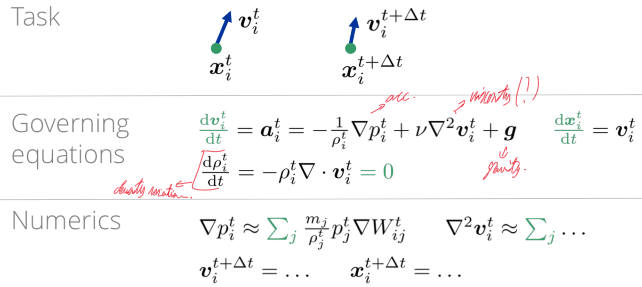
\includegraphics{image1.png}
Pressure is computed by solving a pressure Poisson equation.

\subsection{Rendering aspects}
- Ray Tracing: \\
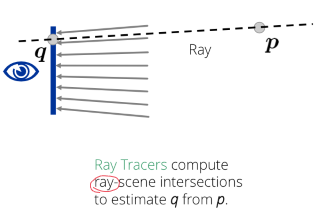
\includegraphics{image4.png}\\
- Rasterization: \\
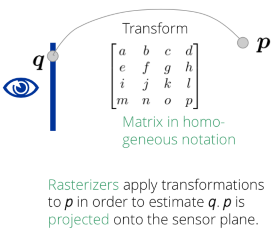
\includegraphics{image5.png}


\subsection{Light}
Photons are characterized by a wavelength within the visible spectrum => color.\\

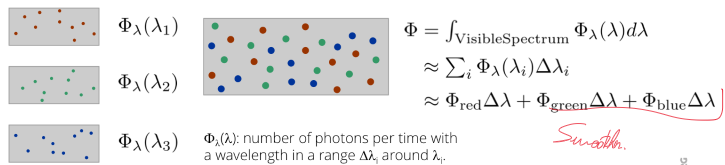
\includegraphics{image2.png}
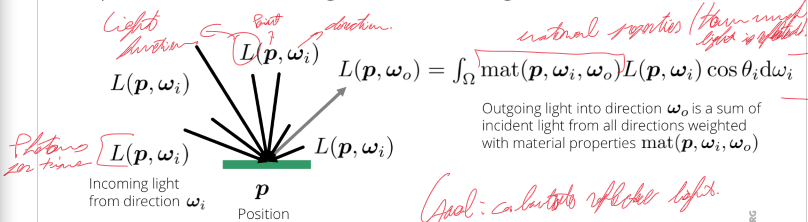
\includegraphics{image3.png}

Rendering -> lookup light transported along rays casted into the scene.
\newpage
\section{Ray Casting}
Rendering problem: visibility/hidden surface problem, object projection onto sensor plane. (Rat-object intersections with ray casting/tracing).\\
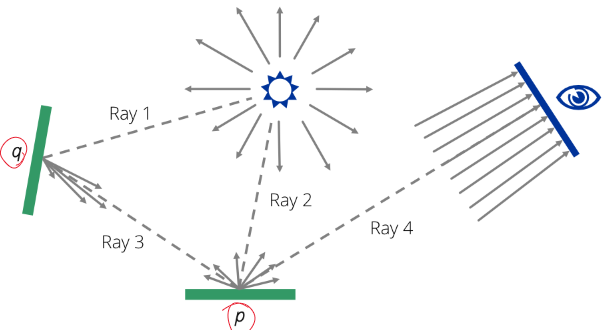
\includegraphics{image6.png}
\textbf{Goal:} to compute ray 4 (incoming light at the sensor considering every riflection).\\
Increasing the number of rays we are considering, we obtain an higher precision (great computationally effort).\\
\textbf{Primary rays: } start/end at sensors\\
\textbf{Secondary rays: } don't start/end at sensors\\
\textbf{Shadow rays: } start/end at sources\\
Primary solve visibility problem, secondary are useful in order to compute light transport.\\
\textbf{Ray casting: }computation of position p (what is visible).\\
\textbf{Ray tracing: }computaiton of light transportd (which colors).\\
Rendering equations to compue incoming light.
\textbf{Concept: }a ray is a half-line specified by an origin o and a direction d => r(t) = o+td with t>=0. We have to compute nearest intersection with all objects.
\subsection{Implicit surfaces}
If p = x,y,z is a surface point => f(x,y,z) = 0.\\
Intersection: f(x,y,z) = f(r(t)) = f(o+td) = 0. All point on a normal surface with offset r satisfy that intersection => n*(p-r) = 0. If d is not orthogonal to n, the intersection can be computed: n*(o+td-r)=0, t=[(r-o)*n]/[n*d].\\
n is given by gradient ( function that compute the variation for unit) of the implicit function (n is the direction with the greater value of gradient).\\
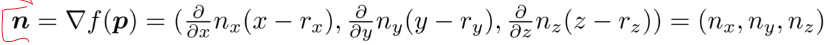
\includegraphics{image7.png}
For quadrics we use the same knowledge expanded to three dimensions (quadratic equations).\\
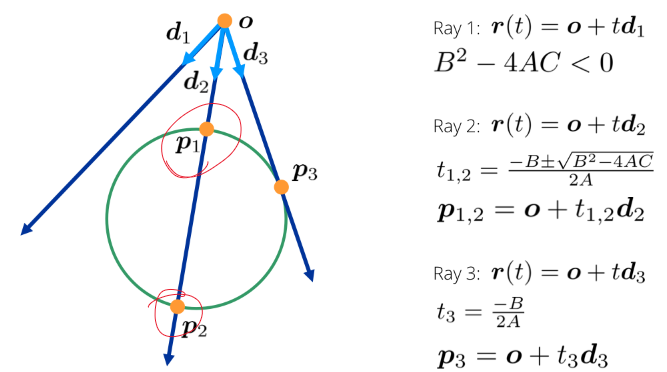
\includegraphics{image8.png}
\subsection{Parametric surfaces}
Represented by functions with 2D parameters: x = f(u,v), y = g(u,v), z = h(u,v)\\
Intersetion can be computer from a non-linear system.\\
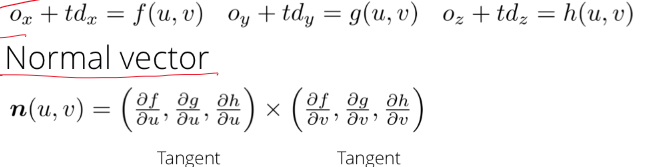
\includegraphics{image9.png}
Parametric representations are used to render partial objects.
\subsection{Combined objects}
\textbf{Compound objects: }union of forms.\\
\textbf{Constructive Solid Geomtry CSG: }combine simple objects to complex geometry using boolean operators.\\
Estimate and analyze all intersections considering intervals inside objects, works for closed surfaces.
\subsection{Triangles}
Popular appoximate surface representation
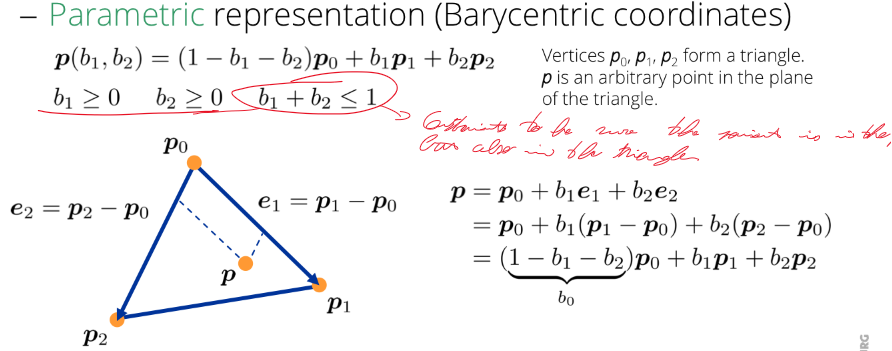
\includegraphics{image10.png}
Intersection: o+td = (1-b1-b2)p0 + b1p1 + b2p2. \\
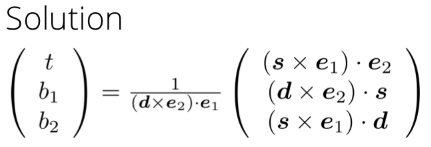
\includegraphics{image11.png}
\subsection{Axis-aligned boxes}
\subsubsection{Axis-Aligned Bounding Box (AABB)}
Simple geometry outside complex geometry, if a ray doesn't intersecate to the simple, surely doesn't intersect the complex. Boxes are represented by slabs. Intersections of rays are analyzed in order to check for ray-object intersection.
Implementations is again done using normal intersection equation.
Overlapping ray intervals indicate intrsections.\\
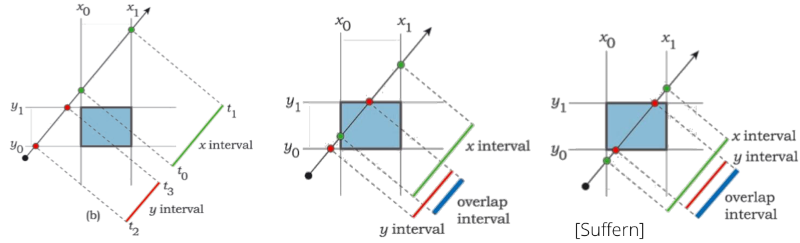
\includegraphics{image12.png}
\subsubsection{Bounding Volume Hierarchies (BVH)}
AABBs combined in a hierarchy way. put smaller boxes recursively. Efficient pruning but memory and pre-processing overhead.
\subsection{Iso-surfaces in grids}
In order to compute intersections on fluid surfaces. Computation is based on density comparison.\\\\
Ray casting is very versatile concept to compute what is visible at a sensor but so expensive for complex geometries.

\section{Shading}
The way to compute color and intensity of what is visible by the sensor. Light is emitted by light sources but is scattered and or absorbed by surface (if dark aborbed, if bright reflected)and media.\\
Radiance: photons per time * area * solid angle (describe how much light is transported).
\textbf{Coloured light }is represented by a 3D vector L: (Lred, Lgreen, Lblue).
\textbf{Coloured objects }are characterized by reflectance coefficient $\rho$ = ($\rho$red, $\rho$green, $\rho$blue). Colours that are in the vector are reflected, otherwise absorbed.\\
We'll use Local Illumination Models that approximately solve the rendering equation.\\
\subsection{Phong Illumination Model}
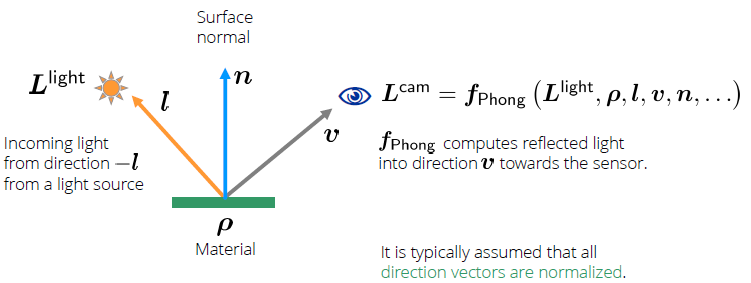
\includegraphics{image13.png}\\
Lsurf is the surface illumination caused by Llight. Lrefl will depend on the object color $\rho$. Lcam is a portion of Lrefl transported to the sensor (will depend on the material).

\begin{theorem}
Illumination strenght at a surface is proportional to the cosine of the angle between l and n.
\end{theorem}
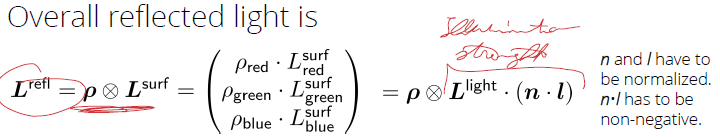
\includegraphics[scale=0.6]{image14.png}\\
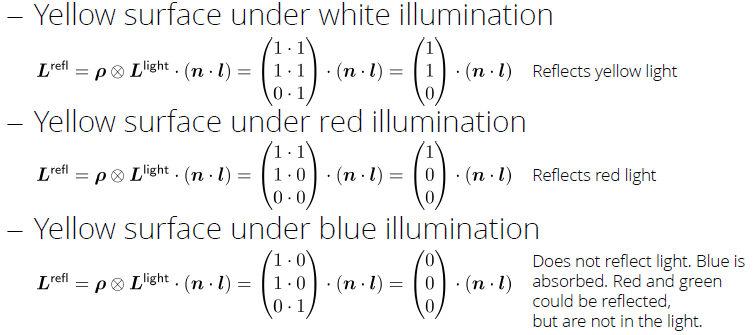
\includegraphics[scale=0.6]{image15.png}\\
Depending on the material, the reflection will be either Diffuse (if Matte) or Specular (if Shiny).\\\\
\subsubsection{Diffuse Reflection}
Matte surfaces reflect light equally into all directions.\\
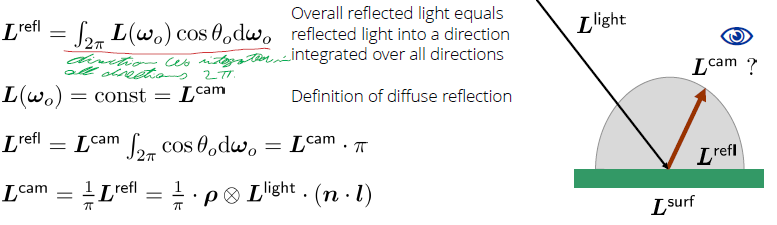
\includegraphics[scale=0.6]{image16.png}\\
\subsubsection{Specular Reflection}
Shiny surfaces reflect light into a small set of dominant directions.\\
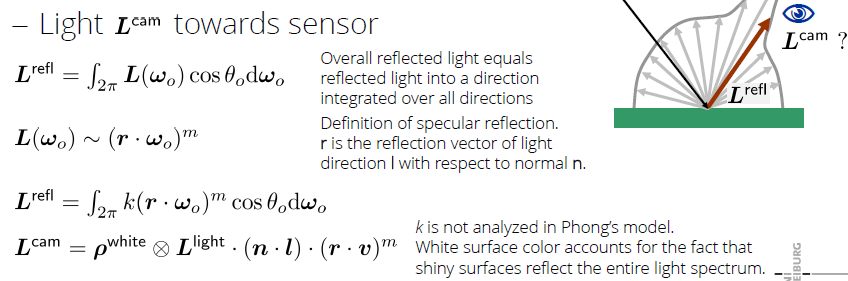
\includegraphics[scale=0.6]{image17.png}\\
Exponent m governs the size of the highlight area. M does not influence the maximal intensity. r can be computed as: r = 2*(l*n)*n-l.\\
According to the Blinn-Phong (Lrefl from a shiny surface) illumination model r = (l+v)/norma(l+v).\\
\subsubsection{Reflection from Ambient Illumination}
Indirect illumination from other surfaces. Reflecte light is: p$\_xor$Lindirect.\\
Lcam = 1/$\_pi$*p$\_xor$Lindirect.
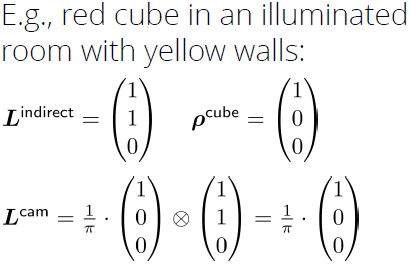
\includegraphics[scale=0.6]{image18.png}
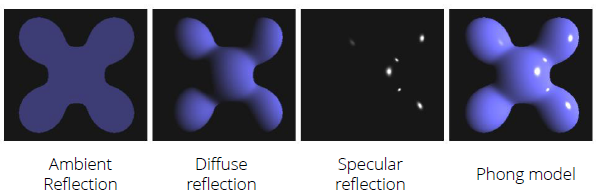
\includegraphics[scale=0.6]{image19.png}\\
\begin{figure}
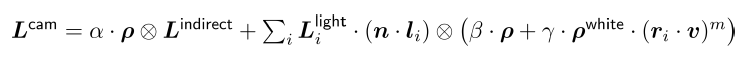
\includegraphics[scale=0.6]{image20.png}
\caption{Total model (coefficients are user-defined)}
\end{figure}
In conclusion Phong is an efficient local computing model and its implementation can be parallelized.Drawbacks: resulting images tend to look less realistic because realistic scenes have more complex illuminations, complex material and non-physical phong parameters cause issues.\\

\subsection{Extensions}
Distances must be considered:\\
1. Between object surface and light source.\\
- Inverse Square Law: Illumination of a surface decreases quadratically with the distance from a light source =\textgreater Lsurf = $(1/r^2)*Llight*(n*l)$.\\
2. Between object surface and viewer.\\
- Fog: It is approximated by a combination of Lcam and Cfog. Lcam,fog = f(d)*Lcam+(1-f(d))*Cfog. f(d) describes the visibility.
\subsection{Shading Models} 
Illumination models can be evaluated per vertex or per fragment.\\
Faces/primitives are characterized by vertices.\\
Projected area of a face onto the sensor is subdivided into fragments.\\
Shading models specify whether the illumination model is evaluated per vertex or per fragment:\\
- If evaluated per vertex, the shading model specifies whether the resulting vertex colors are interpolated across a primitive or not.\\
- If evaluated per fragment, surface normals are interpolated across a primitive.\\
\subsubsection{Well-knows Models}
- Flat shading: evaluation per vertex, fragments are colored with the color of one specific vertex.\\
- Gouraud shading: evaluation per vertex, fragments are interpolated from vertex colors.\\ 
- Phong shading: evaluation per fragment, normals have to be interpolated from vertices to fragments.

\section{Homogeneous Notation}
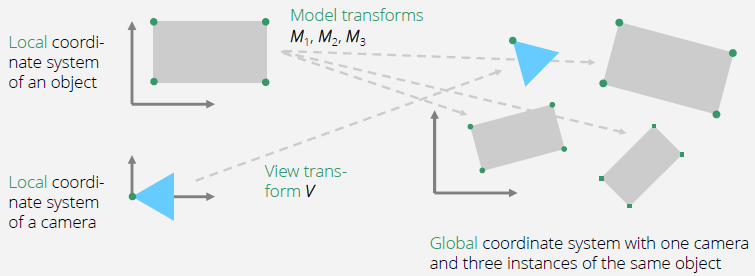
\includegraphics[scale=0.6]{image21.png}\\\\
To transform from view space positions to positions on the camera plane:\\
- Projection transform\\
- Viewport transform\\
Affine trasformatiokns: angles and lengths are not preserved, collinearity, proportions, parallelism are.\\
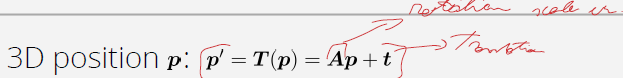
\includegraphics[scale=0.6]{image22.png}\\\\
3x3 matrix A represents linear transformations, 3D vector t represents translation. Using the homogeneous notation, all affine transformations are represented with one matrix vector multiplication.\\
Using the homogeneous notation, transformations of vectors and positions are handled in a unified way.\\
- From Cartesian to Homogeneous:\\
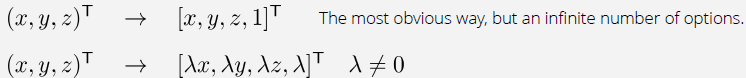
\includegraphics[scale=0.6]{image23.png}\\\\
- From Homogeneous to Cartesian:\\
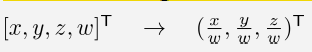
\includegraphics[scale=0.6]{image24.png}\\\\
\begin{figure}
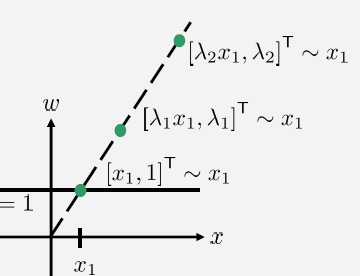
\includegraphics[scale=0.6]{image25.png}
\caption{1D Illustration}
\end{figure}
- General form:\\
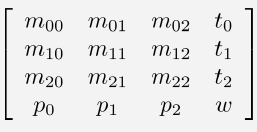
\includegraphics[scale=0.6]{image26.png}\\
m is rotation,scale,shear; t is translation; p for projection; w is the homogeneous component.\\

\subsection{Transformations}
\subsubsection{Translation}
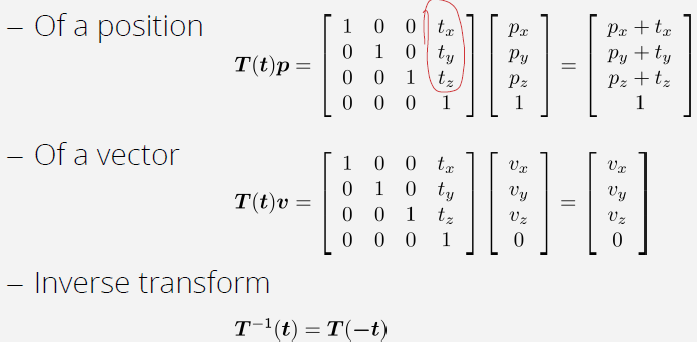
\includegraphics[scale=0.6]{image27.png}\\
\subsubsection{Rotation}
Positive (anticlockwise)\\
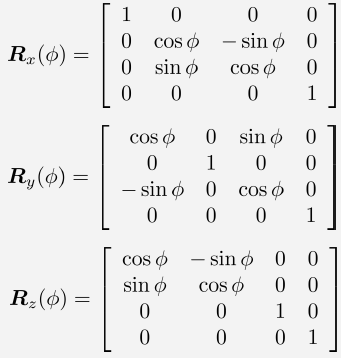
\includegraphics[scale=0.6]{image28.png}\\
\subsubsection{Mirroring}
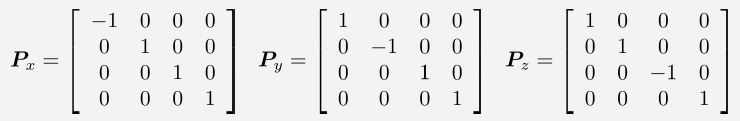
\includegraphics[scale=0.6]{image29.png}\\\\
Rotation and reflection matrices are orthogonal: $RR^T=R^TR=I, R^-1=R^T$
\subsubsection{Scale}
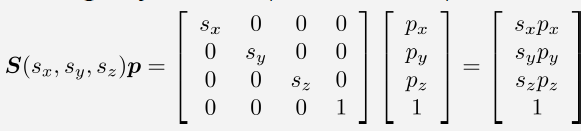
\includegraphics[scale=0.6]{image30.png}\\\\
\subsubsection{Shear}
Offset of one component wrt another component.\\
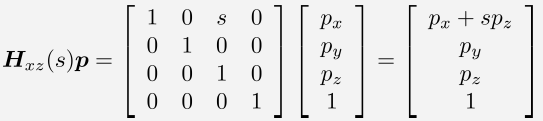
\includegraphics[scale=0.6]{image31.png}\\\\
\textbf{Example:}\\\\
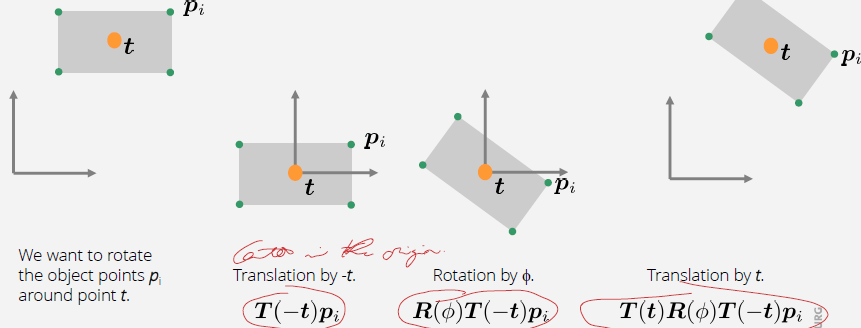
\includegraphics[scale=0.6]{image32.png}\\\\
\subsubsection{Planes and normals}
Planes can be represented by a surface normal n and a point r. All points p with n*(p-r)=0 form a plane.\\
\subsubsection{Basis Transform}
- Translation\\
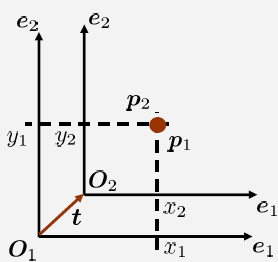
\includegraphics[scale=0.6]{image33.png}\\\\
- Rotation\\
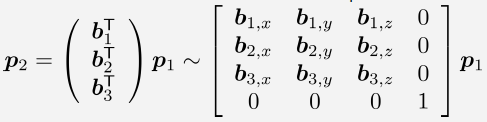
\includegraphics[scale=0.6]{image34.png}\\\\
The view transform can be seen as a basis transform. Placing and orienting the camera is a transformation v.The basis transform is realized by applying $v^-1$ to all objects.\\
Usage of the homogeneous notation is motivated by a unified processing of affine transformations, perspective projections, points, and vectors.All transformations of points and vectors are represented by a matrix vector multiplication.\\

\section{Projection}
Last matrix M row is dedicated to projections and can be used to realize divisions by a linear combination.\\
\begin{figure}
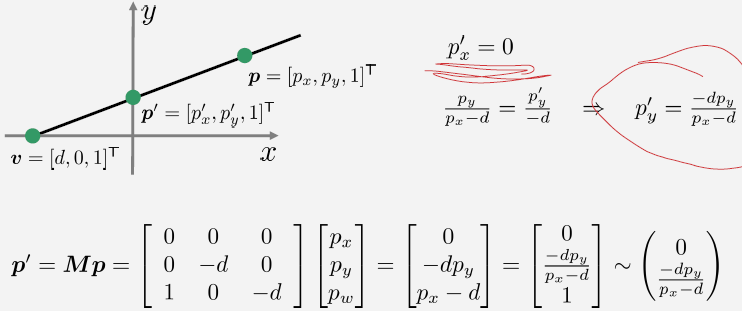
\includegraphics[scale=0.6]{image35.png}
\caption{To compute intersection with the x-axis}
\end{figure}
\subsection{2D projections}
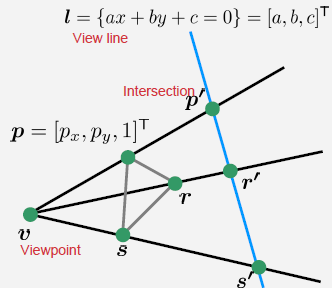
\includegraphics[scale=0.6]{image36.png}\\\\
If the homogeneous component of v is not equal to zero, we have a perspective projection; if v is at infinity, we have a parallel projection.\\
Location of viewpoint and orientation of the viewline determine the type of projection:\\
- Parallel (viewpoint at infinity, parallel projectors).\\
	- Orthographic (viewline orthogonal to the projectors).\\
	- Oblique (viewline not orthogonal to the projectors).\\
- Perspective (non parallel projectors):\\
	- One point (viewline intersects one principal axis).\\
	- Two point (viewline intersects two principal axes, two vanishing points).\\\\
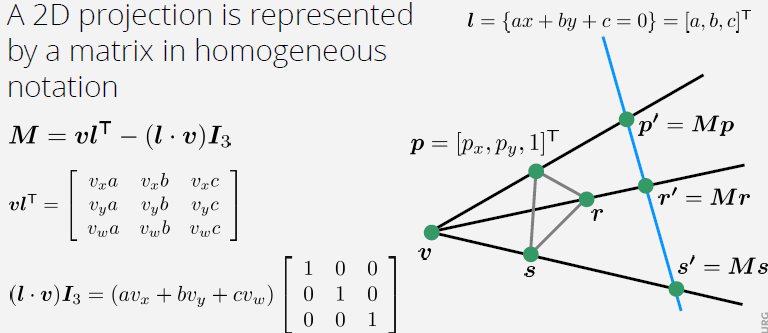
\includegraphics[scale=0.6]{image37.png}\\\\
See other examples on slides.\\\\

\subsection{3D projections}
Same thing expanded to 3D.\\\\
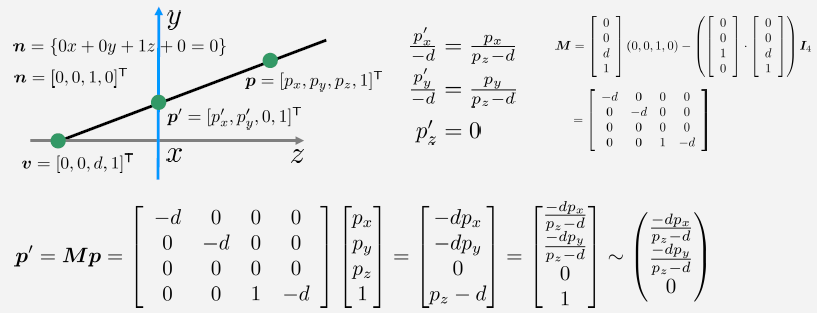
\includegraphics[scale=0.6]{image38.png}\\\\
\section{Projection Transform}
\subsection{Modelview Transformation}
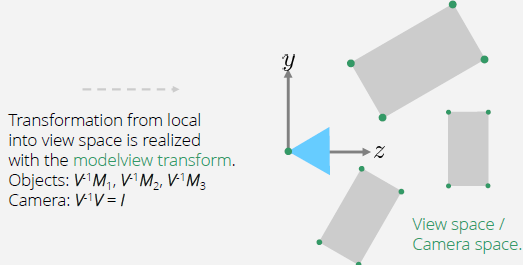
\includegraphics[scale=0.6]{image39.png}\\\\
\subsection{Projection Transformation}
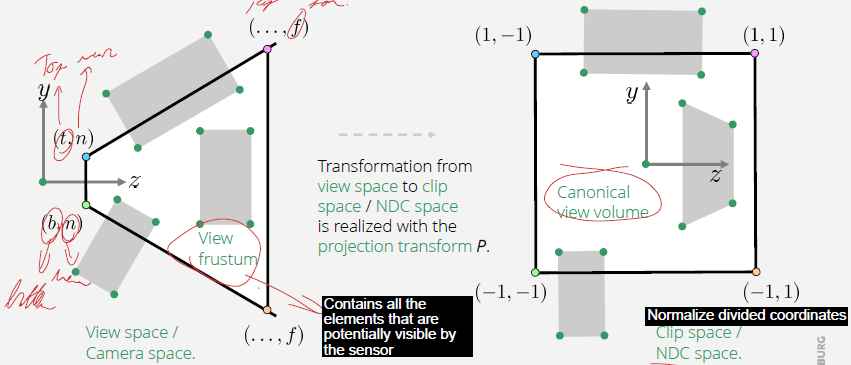
\includegraphics[scale=0.6]{image40.png}\\\\
Why to transform to Clip/NDC? It allows simplified and unified implementations:\\
Culling (exclude non-visible elements), Clipping (exclude non-visible parts of visible elements), Visibility (useful for ray tracing).\\
\subsection{Perspective Projection Transformation}
Maps a view volume/pyramidal frustum (l,r,t,b) to a canonical view volume (-1,1). It is applied to vertices. Maps coordinates to (-1,1) maintaining coherence.\\

- Derivation \\\\
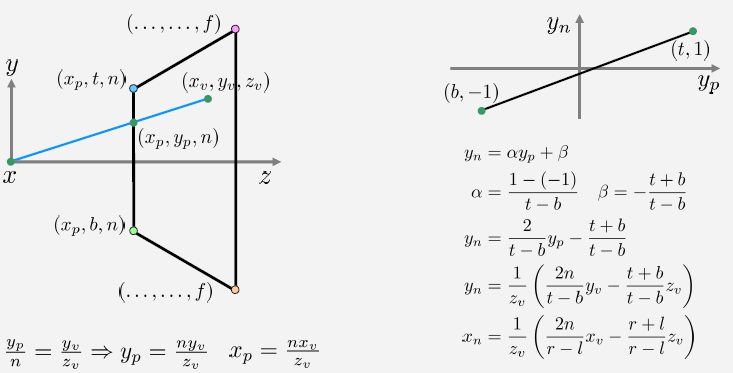
\includegraphics[scale=0.6]{image41.png}\\\\
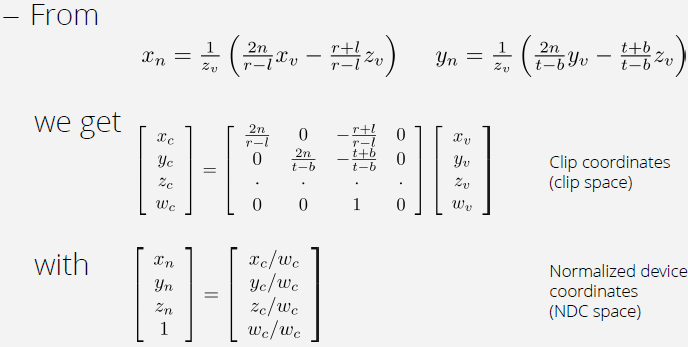
\includegraphics[scale=0.6]{image42.png}\\\\
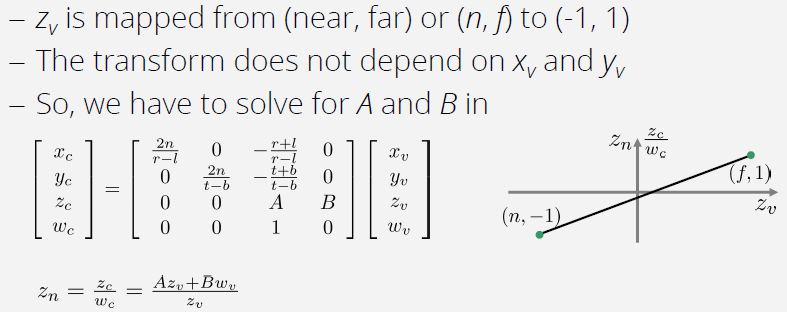
\includegraphics[scale=0.6]{image43.png}\\\\
Then, we can solve A and B and get the complete Projection Matrix
\begin{figure}
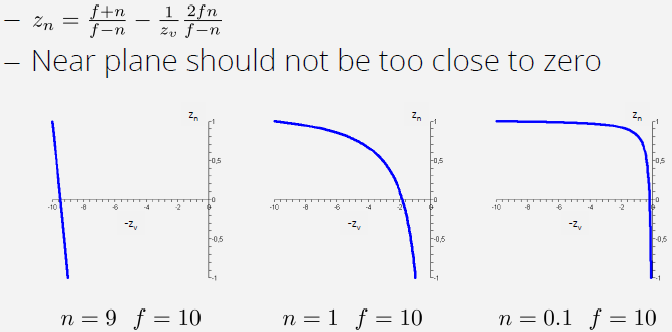
\includegraphics[scale=0.6]{image44.png}
\caption{Non-linear mapping of depth values}
\end{figure}

\subsection{Orthographic Projection}
\begin{figure}
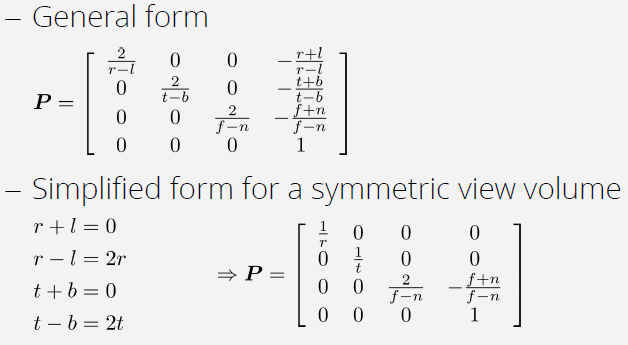
\includegraphics[scale=0.6]{image46.png}
\caption{Matrix general form}
\end{figure}

\section{Typical vertex transformations}
\begin{figure}
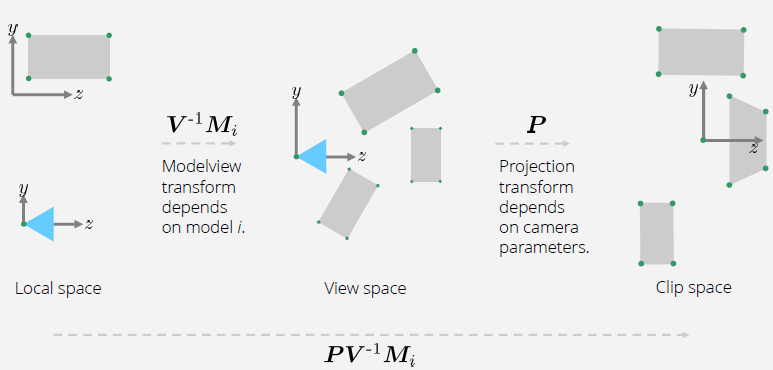
\includegraphics[scale=0.6]{image45.png}\\
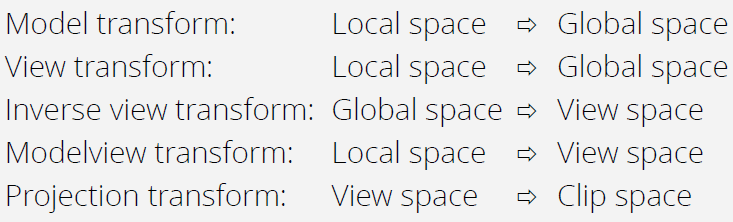
\includegraphics[scale=0.6]{image47.png}\\
\end{figure}
\begin{figure}
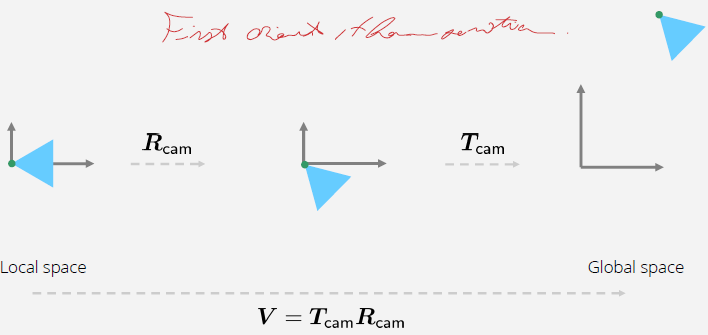
\includegraphics[scale=0.6]{image48.png}
\caption{Camera placement}
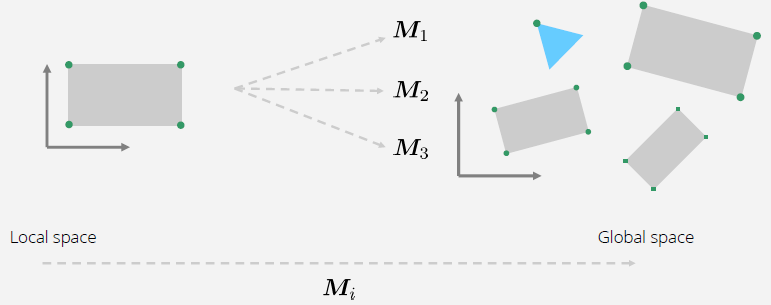
\includegraphics[scale=0.6]{image49.png}
\caption{Object Placement}
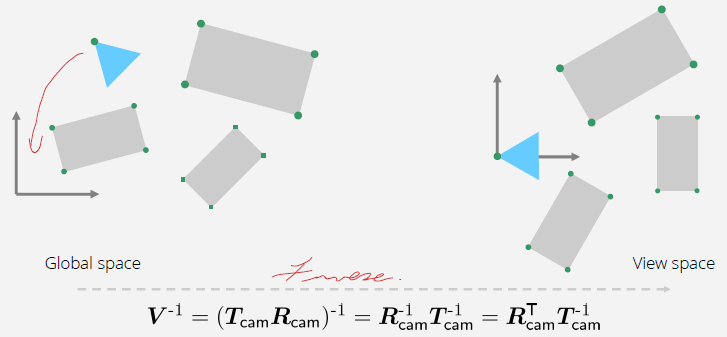
\includegraphics[scale=0.6]{image50.png}
\caption{View Transform}
\includegraphics[scale=0.6]{image51.png}
\caption{Projection transform}
\end{figure}













\end{document}
